\section{Evaluation of classifiers}
\label{sec:eval}

We would like to find the best classification method for Twitter
sentiment.
To evaluate the classification methods, we use three common metrics.
\begin{enumerate}
\item Accuracy = correct guesses / guesses
\item Precision = true positives / (true positives + false positives)
\item Recall = true positives / (true positives + false negatives)
\end{enumerate}
We used accuracy as the criteria for optimization tuning. 

For training and validation, we manually labeled the sentiment of 2800 English
tweets.

\subsection{Subsampling and labeling}

To label as many tweets as possible, we split the workload across the
three authors. Before labeling a large dataset, we took a sample of 280 tweets and had
all three authors label all the tweets. We then compared the labels
(Figure~\ref{fig:agree},
came to agreement on all, and agreed on rules for future labeling.
These rules included labeling obvious spam as neutral and being
conservative about ambiguous tweets. Only two tweets showed complete
disagreement (one vote for each of 3 classes), and these were both judged to
be ambiguous tweets that could have been positive or negative
depending on the latent context.

\begin{figure}[htb]
\begin{center}
  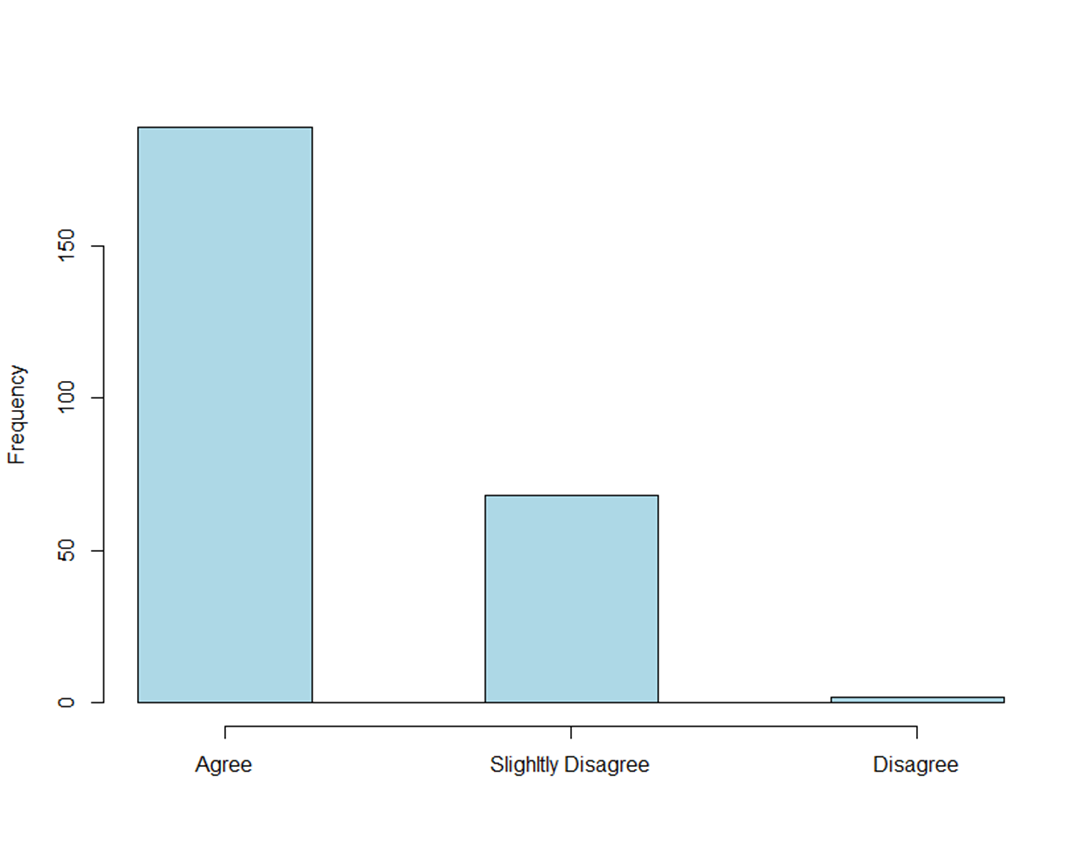
\includegraphics[width=0.9\columnwidth]{figs/agreement280.png}
\begin{minipage}{0.9\columnwidth}
\end{minipage}
\end{center}
\caption{Agreement between 3 manual labelers on 280 random tweets.
    \emph{Disagree} indicates answers differing in polarity.}
\label{fig:agree}
\end{figure}


From 9 collected Markov chains, we took a total of 340,000 samples
from post-burn-in. This yielded 34,054 unique users. We filtered these
users to use only those with registered language English
(lang=``en''), yielding about 20,000 users. From these we took a
uniform sample of 4500 users. For tweets, we used the \emph{status} of
each user (their latest tweet). We found that a large fraction of
registered English users actually tweet at least sometimes in a
different language. To ease the burden of labeling, we ran a language
classifier on the 4500 tweets to provide 2800 likely-English tweets.
These were split into three partitions and labeled according to the
agreed-upon rules. 

We note that this selection introduced bias against
less-connected users, since it is a sample of \emph{unique users} rather than
a subsample of chain draws. The uniform distribution depends on repetitions in the markov chain.
Future labeled subsamples should be true subsamples of the chains, and
we could get unique tweets for a repeated user by examining their
timeline (list of older tweets). Another bias is that the sample was
overly aggressive and included some users drawn before convergence. Overall, our labeled tweets dataset may reflect
the true Twitter population with some bias. This should not affect
accuracy evaluations, but it \emph{will} affect certain priors learned by the
classifiers; so for application of the classifiers, a more disciplined
subsample of our uniform sample should be taken.

\subsection{Comparison}

We applied
the six methods to the labeled dataset of 2800 tweets. For
unsupervised methods, we just computed accuracy from labeled tweets
that landed in the wrong class. For supervised methods, we used 5-fold
cross validation. The three supervised learning methods besides the
baseline have the highest accuracy (see Table~\ref{table:compare}).

\begin{table}[htb]
\center
\begin{tabular}{|c|c|}
    \hline
Method & Accuracy\\
\hline
SVM & 65\% \\
\hline
KNN & 64\% \\
\hline
LDA & 62\% \\
\hline
NB with word list & 49\% \\
\hline
KMeans with PCA & 40\% \\
\hline
NB (supervised) & 34\% \\
\hline
\end{tabular}
\caption{Classification Accuracy of Different Methods}
\label{table:compare}
\end{table}

Figure~\ref{fig:cob} compares the top three methods in terms of all
three metrics (accuracy is implicit). SVM and KNN perform poorly on
recall as they conservatively label too many sentimental tweets as
neutral. On the other hand, LDA is more aggressive about labeling
sentiments, sacrificing precision on sentimental tweets for better
recall on sentimental tweets. Given that
most mistakes are between the boundaries with neutral, a higher recall
rate might be desirable for looking at the proportion of Twitter users
between all three classes, while a higher precision might be desirable for
looking at the proportion of Twitter users that are negative versus
positive.


\begin{figure}[htb]
\begin{center}
  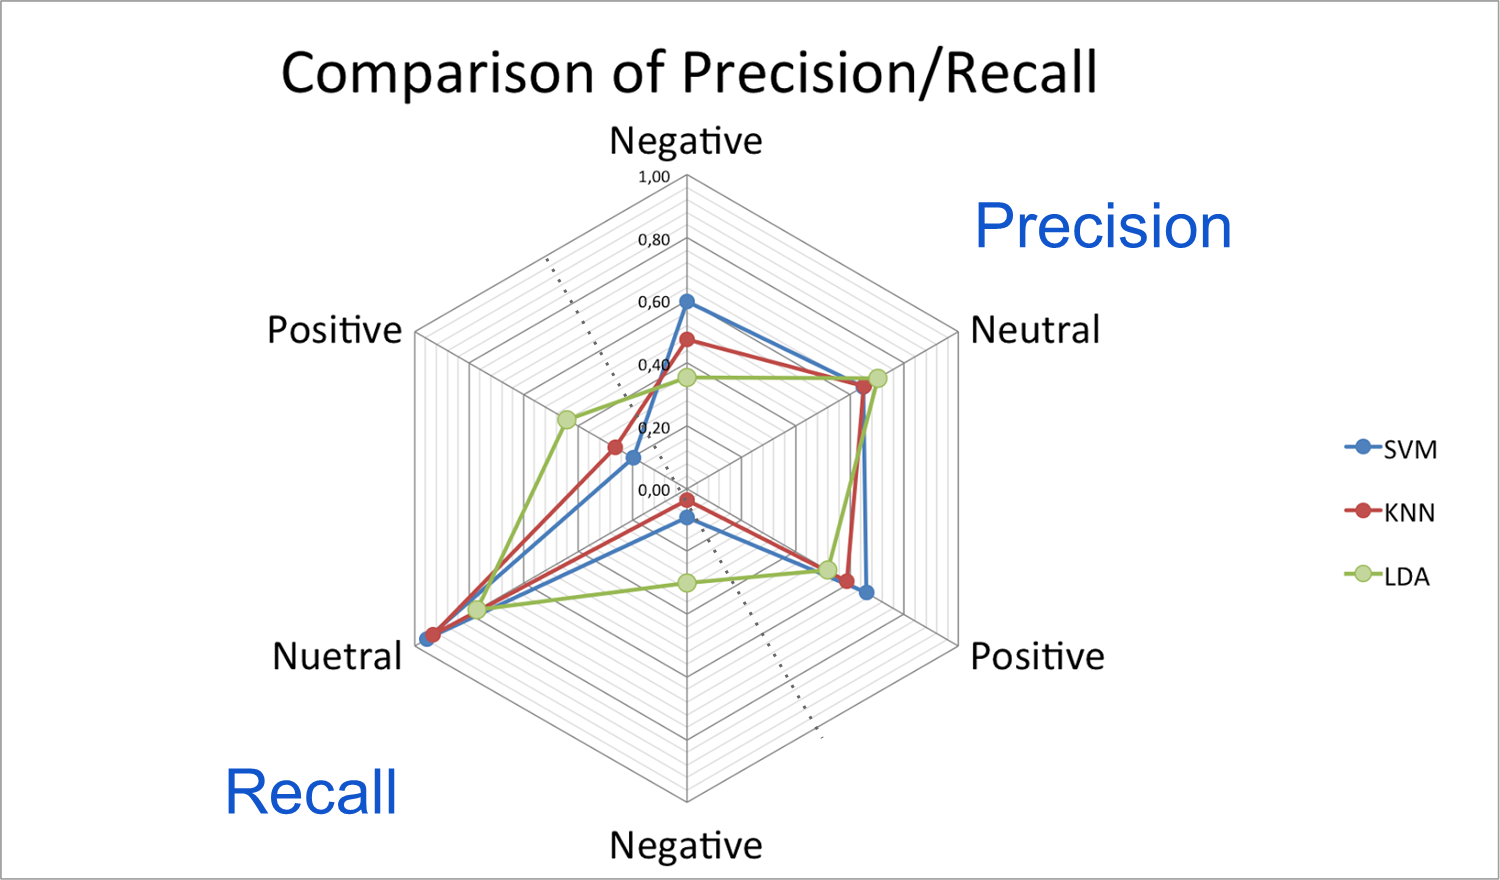
\includegraphics[width=0.9\columnwidth]{figs/cobweb.png}
\begin{minipage}{0.9\columnwidth}
\end{minipage}
\end{center}
\caption{Precision and recall for the most accurate methods: SVM, KNN,
    and LDA.}
\label{fig:cob}
\end{figure}


%%%\begin{table*}[htb]
%%%\center
%%%\begin{tabular}{|c|c|c|c|c|c|c|}
%%%\hline
%%%Method&SVM & KNN & LDA & NB with word list & PCA with K-Means & NB (supervised)\\
%%%\hline
%%%Accuracy& 65\% & 64\% & 62\% & 49\% & 40\% & 34\% \\
%%%\hline
%%%\end{tabular}
%%%\caption{Classification Accuracy of Different Methods}
%%%\end{table*}




















